\section{Implementation}
In diesem Kapitel beschäftigen wir uns mit der Implementation und mit dem Aufbau von Grafana, sodass wir \gls{Cyberangriff} nach dem \gls{mitre} Matrix erkennen können. Wir gestalten unser Arbeitslabor mit \gls{container} und \glsfirst{vm}, wie in dem folgenden Diagramm:

\begin{figure}[H]
   \centering
   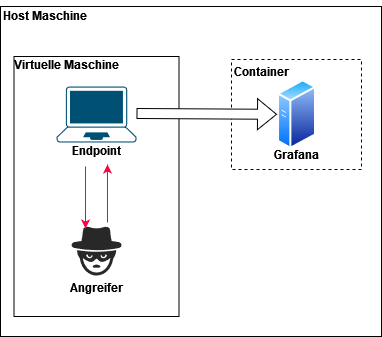
\includegraphics[width=0.8\textwidth]{assets/Arbeitslabor.drawio.png}
   \caption{Aufbau unseres Arbeitslabors \\Quelle: Eigene Quelle}
   \centering
\end{figure}

Von unserem Aufbau zielen wir, die Aufnahmen und Anpassung der Logdateien für Grafana, die Musterkerennung für die ausgewählten \glsplural{Cyberangriff} und schließlich die Warnmeldung für die Endnutzer, sodass sie sich für entsprechende Sicherheitsmßnahmen entscheiden können. 

\newpage
Der gewünschte Ablauf ist in dem folgenden Diagramm dargestellt:

\begin{figure}[H]
   \centering
   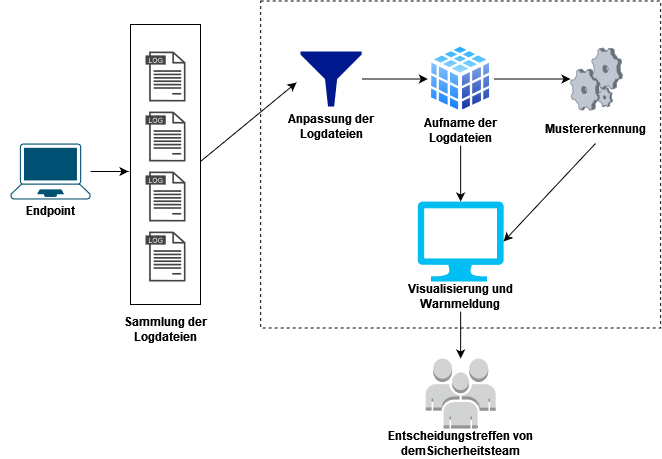
\includegraphics[width=1\textwidth]{assets/Ablauf_grafana.drawio.png}
   \caption{Erwarteter Ablauf von der Datensammlung bis zur Warnmeldung von \glsplural{Cyberangriff} \\Quelle: Eigene Quelle}
   \centering
\end{figure}

\subsection{Angriffserkennung anhand der Mitre ATT\&CK Matrix\textregistered}
Es gibt verschiedene Methode und Framework zur Vermeidung, Erkennung, und Unterbrechung von \glsplural{Cyberangriff}. \glsfirst{owasp}, \glsfirst{CKC} und \gls{mitre} Matrix sind einige Bespiele von denen, die \gls{SOC}-Teams verwenden, um Sicherheit von Systemen und/oder Netzwerken zu gewährleisten. Da die Richtlinien und Fokus von diesen Frameworks sich unterscheiden können und deswegen anderen Aufbau von unserer Struktur verlangen wurden, entschieden wir uns für die Anwendung von der \gls{mitre} Matrix für die Erkennung der \glsplural{Cyberangriff} besonders, weil dieser Framework auch an Splunk integriert ist.

\newpage
Die \gls{mitre} Matrix hat folgende Hauptnutzung \citep{Mitre_Started}:

\begin{itemize}[noitemsep]
   \item Erkennung und Analyse von Angriffstechnik
   \item	strukturierte Datensammlung über Bedrohungen
   \item	Emulieren von \glsplural{Cyberangriff} für die Anwendung an Angriffsübungen
   \item	Systemhärtung und Verbesserung der Verteidigungsmaßnahmen
\end{itemize}

Die Matrix bietet eine umfangreiche Verwendung für Unternehmen und für \gls{SOC}-Team an, um ihre wertvollen Ressource schützen und ihre Fachkenntnisse über \gls{Cybersicherheit} zu erweitern \citep{Hazel_howtousemitre}. Hier konzentrieren wir uns auf die Entwicklung und auf die Implementierung einer Methode für die automatische Erkennung und Analyse von Angriffstechnique in Grafana.

Die \gls{mitre} Framework besteht aus 14 Taktik. Zu jedem Taktik gehören Technique, die ihrerseits in Subtechniques aufgeteilt sind. Jede Subtechnique wird mit Beispielen, Härtungsmaßnahmen und Erkennungsregeln dargestellt. Die nächste Abbildung zeigt, wie diese Struktur aufgebaut ist: 

\begin{figure}[H]
   \centering
   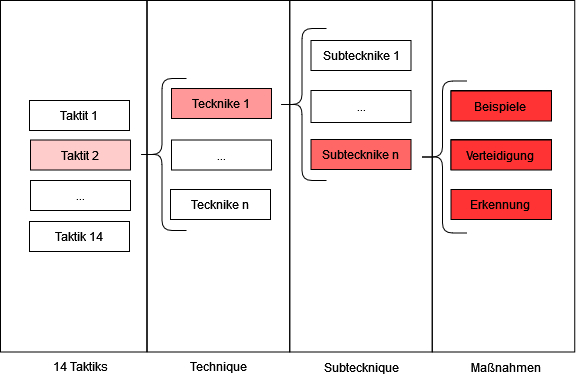
\includegraphics[width=0.8\textwidth]{assets/Mitre_structure.drawio.png}
   \caption{Struktur der Mitre Matrix \\Quelle: Eigene Quelle und \citep{Mitre_Started}}
   \centering
\end{figure}

\newpage
Die 14 Tactics sind folgende:
\begin{itemize}[noitemsep]
   \item Informationssammlung für zukünftige Angriffe 
   \item	Entwicklung von Ressource von Angreifer
   \item Erster Zugang zum Opfersysteme 
   \item Ausführung von bösartigen Coden
   \item Beharrlichkeit von System
   \item	Privilegienausweitung
   \item Vermeidung von Verteidigungssysteme
   \item Zugang zu Anmeldedaten
   \item Umgebungserkennung
   \item Seitliche Bewegung zu anderem Systemen innerhalb des Angriffsziels
   \item interne Informationssammlung
   \item Steuerung und Kontrolle (C2 - Command and Control im Original)
   \item Datenextrahierung 
   \item	Auswirkung auf die Integrität
\end{itemize}


\subsection{Auswahl des Angriffes}
In dieser Arbeit beschäftigen wir uns mit dem Tactic \quotes{Zugang zu Anmeldedaten} und deren Technique \gls{bruteforce}. Diese Technique ist in vier Subtechnique aufteilt:

\begin{itemize}[noitemsep]
   \item Erraten von Anmeldedaten 
   \item	Entschlüsselung von \glsplural{hash}
   \item \textit{\gls{stuffing}}
   \item \textit{\gls{spraying}}
\end{itemize}

Da unser Ziel hier ist Grafana, zu benutzen, um Angriffe zu erkennen, entschieden wir uns für einen einfachen reproduzierbaren Angriff, die weniger Ressource verlangt. In diesem Fall, lässt sich \gls{bruteforce} einwandfrei mit zwei \glsplural{vm} darstellen. Für diesen Angriff benutzen wir die Subtechnique \quotes{Erraten von Anmeldedaten und \textit{\gls{stuffing}}}, da sie ähnliche Erkennungmethode haben. Hier schließen wir auch die anderen Maßnahmen aus.

Die nächste Abbildung zeigt den Umfang unseres Implementationsversuchs:
\begin{figure}[H]
   \centering
   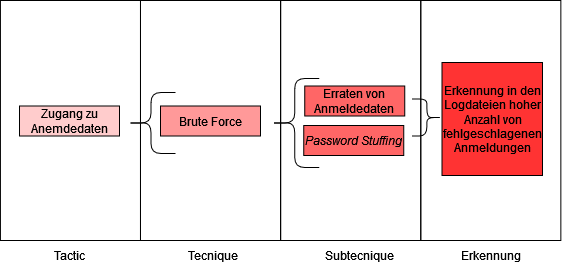
\includegraphics[width=0.8\textwidth]{assets/T1110.drawio.png}
   \caption{Analysestruktur für diese Arbeit \glsplural{Cyberangriff} \\Quelle: Eigene Quelle und \citep{Mitre_t1110}}
   \centering
\end{figure}

\subsection{Installation und Erstellung von Logdateien}
In diesem Abschnitt fokussieren wir uns auf folgenden Punkten:

\setlist{nolistsep}
\begin{enumerate}[noitemsep]
   \item Installation von Grafana Loki mit \gls{container}
   \item	Einrichtung der \glsplural{vm} für Opfersystem und Angreifen
   \item	Angriffsssimulation für die für die Generierung von Logdateien
   \item Weiterleitung der Logdateien vom Opfersystem (\gls{Endpoint}) zu Grafana Loki
\end{enumerate}

Die Installation und Anwendung können entweder mit dem \gls{GUI} oder mit der Kommandozeilen durchgeführt werden. In dieser Arbeit benutzen wir die Kommandozeile. 

\newpage
\subsubsection{Installation von Grafana Loki mit \gls{container}}
Grafana lässt sich mit folgenden Kommandos in Docker \gls{container} ausführen:

\begin{spverbatim}
wget https://raw.githubusercontent.com/grafana/loki/v2.8.0/cmd/loki/
loki-local-config.yaml -O loki-config.yaml

docker run --name loki -v <local-path>:/mnt/config -p 3100:3100 
grafana/loki:2.8.0 --config.file=/mnt/config/loki-config.yaml

wget https://raw.githubusercontent.com/grafana/loki/v2.8.0/clients/cmd
/promtail/promtail-docker-config.yaml -O promtail-config.yaml

docker run -v <local-path>:/mnt/config -v /var/log:/var/log --link loki 
grafana/promtail:2.8.0 --config.file=/mnt/config/promtail-config.yaml
\end{spverbatim}

Die obigen Kommandos haben folgende Bedeutungen:
\begin{enumerate}[noitemsep]
   \item Herunterladen der Konfigurationsdatei von Grafana Loki
   \item Ausführung der Loki \gls{container}, Nutzung des lokalen und externen \glsplural{port} 3100 für die Netzwerkverbindung und Verwendung der heruntergeladenen Konfigurationsdatei
   \item Herunterladen der Konfigurationsdatei von Promptail
   \item Ausführung der Promptail \gls{container}, Verbindung zwischen diesen und den Loki \gls{container} und Verwendung der heruntergeladenen Konfigurationsdatei
\end{enumerate}

Für spezifische Versionen oder andere weitere Einstellungen bietet die Dokumentation umfangreiche Möglichkeiten an \citep{Grafana_run}.

\newpage
\thispagestyle{lscape}
\begin{landscape}
   Nach der Ausführung des Kommandos ist die Anwendung schon benutzbar, wie in dem folgenden Screenshot:
   \begin{center}
      \begin{figure}[H]
         \centering
         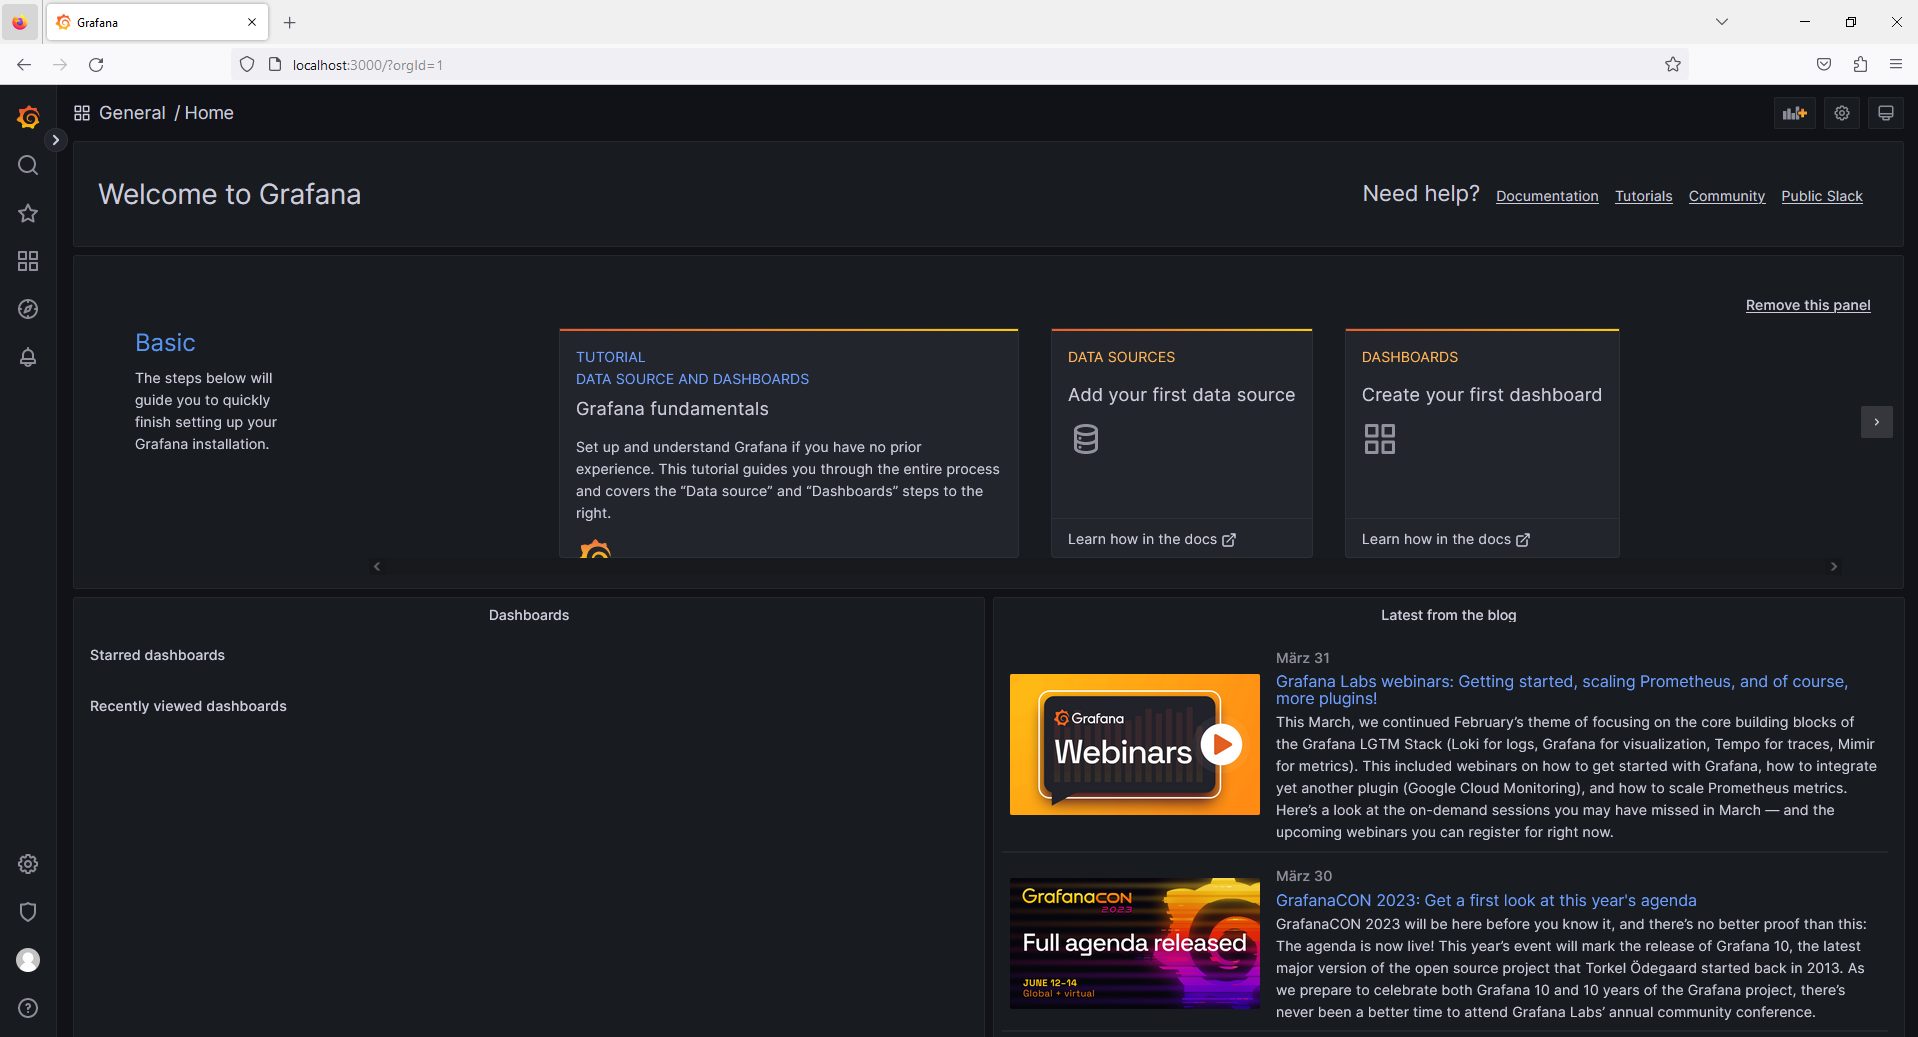
\includegraphics[width=1.3\textwidth]{assets/Installation_Grafana.png}.
         \caption{Screenshot der Willkommensseite von Grafana Loki\\Quelle: Eigene Quelle und \citep{Grafana_Logs}}
         \centering
      \end{figure}
   \end{center}
\end{landscape}

\subsubsection{Einrichtung der \glsplural{vm} für Opfersystem und Angreifen}
Die beiden \glsplural{vm} sind \quotes{\gls{kali} vorgebaute \glsfirst{vm}} und \quotes{\gls{ubuntu} Server 22.04.2} in ihren standardmäßigen Einstellungen. Beiden Maschinen lassen sich aus der jeweiligen Schritte Dokumentation einwandfrei installieren \citep{kali_vm} und \citep{Ubuntu_server}.

Für das Opfersystem entschieden wir uns für das Passwort \quotes{qwertz}. Laut einer Umfrage gehört dieses Passwort zu den zehn meisten verwendeten Passwort in Deutschland \citep{silicon_passwort}.  

Für die Durchführung von \gls{spraying} erstellen wir folgende Benutzer und Passwörterkombinationen:
\begin{verbatim}
   admin:123456
   user1:passwort
   user2:abc123
   user3:qwertyuiop
\end{verbatim}

\subsubsection{Angrifsssimulation für die für die Generierung von Logdateien}
Für den Angriff verwenden wir folgenden Tools:
\begin{itemize}[noitemsep]
   \item	\glsfirst{ssh}
   \item \gls{hydra}
\end{itemize}

In diesem Szenario schickt \gls{hydra} gleichzeitig mehrere Authentifizierungsversuche zum Opfersystem, um eine \gls{ssh} Verbindung mit dem Opfersystem zu erstellen. Das Tool verwendet ein sogenanntes Wörterbuch mit verschiedenen Einträgen, die als Passwörter dienen. Für unseren Test benutzen wir die bekannten Datei \gls{rockyou} Datei. 

\newpage
Die nächste Abbildung zeigt, wie \gls{stuffing} abläuft:

\begin{figure}[H]
   \centering
   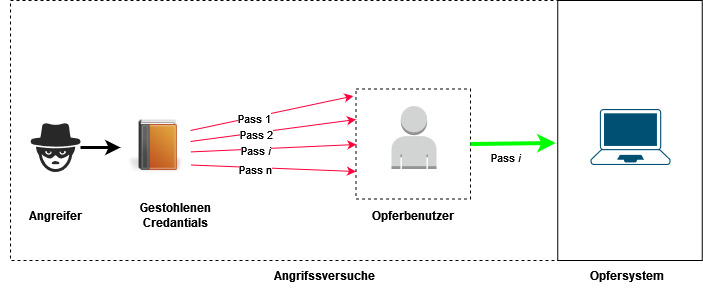
\includegraphics[width=0.8\textwidth]{assets/Stuffing.jpg}
   \caption{\textit{\gls{stuffing}}\\Quelle: Eigene Quelle und \citep{Nguyen_stuffing}}
   \centering
\end{figure}

Das folgende Kommando wurde gegen das Angreifersystem für \gls{stuffing} ausgeführt:
\begin{spverbatim}
   hydra -l test -P rockyou.txt [Adresse von Opfersystem] ssh -V -t 4
\end{spverbatim}

Das gesamte Kommando lässt sich folgendes erklären \citep{kali_hydra}:
\begin{spverbatim}
   -l: Spefizikation der Benutzername, den wir Angreifen
   -P: Auswahl der Datei mit bekannten Passwörter
   ssh: Auswahl der Anwendung, die wir angreifen wollen
   -V: Ausgabe ausführlicher Information über die Durchführungen, wie Versuche, Fehlermeldungen und Erfolge
   -t 4: Anzahl von gleichzeitigen Verbindungen
\end{spverbatim}

\newpage
Für \gls{spraying} benutzen wir folgendes Kommando:
\begin{verbatim}
   hydra -L username.txt -P rockyou.txt [Adresse von Opfersystem] ssh -V -t 4
\end{verbatim}

Das \quotes{-L} (großes \quotes{L}) ist der einzige neue Parameter. Er dient für die Auswahl einer Textdatei mit einer Liste von Benutzername.

Ein \gls{spraying} Angriff sie wie folgende aus:
\begin{figure}[H]
   \centering
   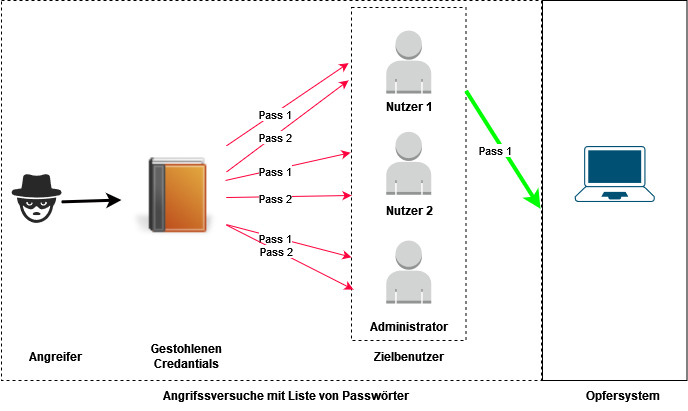
\includegraphics[width=0.8\textwidth]{assets/Spraying.jpg}
   \caption{\textit{\gls{spraying}}\\Quelle: Eigene Quelle und \citep{Swathi_spraxy}}
   \centering
\end{figure}

\subsubsection{Weiterleitung der Logdateien vom Opfersystem (\gls{Endpoint}) zu Grafana Loki}
aaaaaaaaaaaaaaaaaaaaaa

\subsection{Aufbau der Erkennungsregel für den ausgewählten Angriff}
Der \gls{bruteforce} lässt sich durch die Anzahl des fehlgeschlagen Anmeldungsversuchs erkennen \citep{Selvaganesh_SplunkBruteForce}. Wir bearbeiten eine Situation, in der es keine Gegenmaßnahmen, wie Kontosperre nach \textit{n} beliebigen Versuchen oder \gls{mfa}, implementiert sind. Das folgende Aktivitätsdiagramm stellt einen allgemeinen Ablauf eines Anmeldungsverfahrens dar:

\begin{figure}[H]
   \centering
   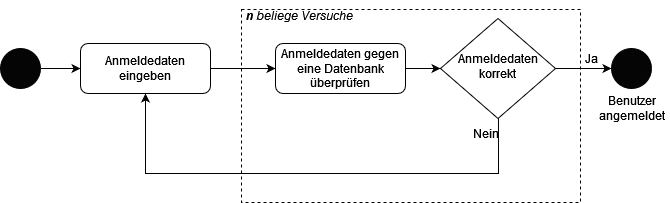
\includegraphics[width=0.8\textwidth]{assets/Anmeldeverfahren.drawio.png}
   \caption{Allgemeiner Ablauf eines Anmeldungsverfahrens \\Quelle: Eigene Quelle und \citep{Selvaganesh_SplunkBruteForce}}
   \centering
\end{figure}

\textcolor{red}{\textbf{Regel von SPLUNK hinzufügen, wie sollten unsere Regel aussehen}}

\textcolor{red}{\textbf{statische vs dinymische Regel}}





\subsection{Bewertung der Daten in Grafana}
Hinzufügen der Logdateien und Erstellung von Regeln zur Erkennung des Angriffes
Diagramm der Nutzung von Grafana

\subsection{Normalisierung der Logdateien mit Zeek}
Diagramm der Nutzung von Grafana und Zeek

Hier werden die Schritte für die Installation und Sammeln von Daten beschrieben.

- Implementation in Container %https://rdr-it.com/elk-installation-configuration-un-siem-docker/


\subsection{Sammlung von Server-Log Dateien}

\subsection{Normalisierung der Log-Dateien}





